%===============================================================================
% Advanced IPC and I/O.
%===============================================================================

\section{Advanced IPC and I/O}

%References
%- [mcdougall] 4.8 Solaris Doors
%- [posix.1d]

%===============================================================================
\subsection{Advanced IPC and I/O}

\begin{itemize}
\item (Slightly) More on the \texttt{ioctl(2)} System Call
\item Doors Interface as a Lightweight RPC
\item Passing File Descriptors Between Processes
\item POSIX Real-time Signals
\item Asynchronous POSIX I/O
\item Existing Means of Creating a New Process, and new ones:
	\begin{itemize}
	\item \texttt{popen()} with \texttt{pclose()}
	\item \texttt{posix\_spawn()}
	\end{itemize}
\end{itemize}

%===============================================================================
\subsection{Known Means of IPC}

\begin{itemize}
\item oldest (pre-1980) UNIX systems
	\begin{itemize}
	\item signals
	\item process tracing
	\item files and shared file offests
	\item pipes
	\end{itemize}
\item then:
	\begin{itemize}
	\item named pipes (FIFOs)
	\item file locks
	\item sockets
	\item (System V IPC) semaphors, messages, shared memory
	\item POSIX version of semaphores, messages, and shared memory
	\end{itemize}
\end{itemize}

\begin{itemize}
\item ,,Known'' means known to you from [\myun\myix-prog-I]. Those are \emsl{14
different mechanisms} of how processes can communicate with each other.
\item And there are more:
	\begin{itemize}
	\item doors
	\item passing file descriptors between processes
	\item and probably something else...
	\end{itemize}
\item Process tracing is done today using \texttt{/procfs}, which might be
considered an IPC over files. However, there was, and sometimes still is,
\texttt{ptrace()} call, usually a system call, that allowed one process to debug
another one. Debugging means setting and clearing breakpoints, and reading and
writing the other process's address space.
\item {} [\myun\myix-prog-I] introduced System V IPC semaphores only, and just
mentioned messages and shared memory, including its POSIX equivalents. However,
it's recommended to use the POSIX calls. In general, mostly you do not need
messages and shared memory since you can use pipes or sockets for data passing,
and \texttt{mmap(2)} for memory sharing (which with \texttt{MAP\_ANON} does not
even need a file descriptor at all).
\end{itemize}

%===============================================================================
\subsection{ioctl(2)}

\begin{itemize}
\item a catchall for I/O operations
	\begin{itemize}
	\item when there is no specific funtion for particular I/O, it usually ends
	  up in \texttt{ioctl()}
	\end{itemize}
\item terminal I/O is (was) the biggest user of this function
	\begin{itemize}
	\item however, POSIX introduced separate functions for terminal handling
	\end{itemize}
\item easy access to kernel through device drivers
\item UNIX spec includes \texttt{ioctl()} only as an extension for
dealing with STREAMS devices, but it is used heavily elsewhere as well
\item and \emsl{why} is \texttt{ioctl()} so convenient? Because you give it a
command (\texttt{int}) and then a variable number of other parameters.
\end{itemize}

\begin{itemize}
\item \texttt{int ioctl(int fd, int request, /* arg */ ...);}
\item The command (request) is interpreted by the driver so if you write your
own driver, you interpret the commands as you wish, and most probably you define
your own macros for your commands, and put those macros in a public header file
for the driver.
\item STREAMS is a mechanism on some UNIX implementations that allow character
device drivers to be implemented in a modular fashion. Some systems extended
this idea. For example, pipes are implemented on top of STREAMS on Solaris.
Anyway, users usually do not have to care about that. See page
\pageref{IOCTLEXAMPLE} for an example.
\item We just cannot invent another system calls as we see fit so we use
\texttt{ioctl()} for that.
\end{itemize}

%===============================================================================
\subsection{Example: \texttt{/dev/crypto} on Solaris}

\begin{itemize}
\item Solaris Cryptographics Framework provides crypto services to users and
applications
\item it has a user level and a kernel level part. You always link to
\texttt{libpkcs11.so} library.
\item \texttt{libpkcs11.so} can utilize HW crypto through the
\texttt{pkcs11\_kernel.so} library
\item your application $\rightarrow$ \texttt{libpkcs11.so} $\rightarrow$
\texttt{pkcs11\_kernel.so} $\rightarrow$
\texttt{ioctl()} on \texttt{/dev/crypto}
	\begin{itemize}
	\item ie. through \texttt{/dev/crypto} pseudo driver we get to the
	kernel from the user space
	\end{itemize}
\end{itemize}

\begin{itemize}
\item The kernel part of the Crypto Framework takes care of HW crypto cards, for
example.
\item In the user level part, you can utilize the software crypto providers
working completely in user level. That means that all the implementation is
provided by a software library (aka ,,software provider''). However, what we are
interested here is the kernel part of the Crypto Framework.
\item \texttt{CRYPTO\_DEVICE} is defined as \texttt{/dev/crypto}:\\
\url{http://src.opensolaris.org/source/xref/onnv/onnv-gate/usr/src/lib/pkcs11/pkcs11\_kernel/common/kernelGlobal.h}
\item It is opened here:\\
\url{http://src.opensolaris.org/source/xref/onnv/onnv-gate/usr/src/lib/pkcs11/pkcs11\_kernel/common/kernelGeneral.c}
\item And it is used through \texttt{ioctl()} here, for example, to perform an
encryption:\\
\url{http://src.opensolaris.org/source/xref/onnv/onnv-gate/usr/src/lib/pkcs11/pkcs11\_kernel/common/kernelEncrypt.c}
\item \label{DEV_POLL} Another example from Solaris -- you know \texttt{poll()}
and \texttt{select()} calls. While \texttt{poll()} is preferred (you should know
why), it still has issues. For example, polling thousands of file descriptors
will little activity on them means that we must pass all those structures to
kernel for every call. It is better to use \texttt{/dev/poll} pseudo device
which provides what \texttt{poll()} can do for you, and more. It keeps all the
information about polled descriptors in kernel memory, for example. And you use
\texttt{ioctl()} to manipulate \texttt{/dev/poll}, of course. You can read the
following documents to get more information:\\
\url{http://developers.sun.com/solaris/articles/polling\_efficient.html}\\
\url{http://developers.sun.com/solaris/articles/using\_devpoll.html}
%\item TODO: have a simple pseudo driver, and have readers to implement a new
%\texttt{ioctl} command. You can see source code for \texttt{/dev/crypto} on how
%to create entry points for individual \texttt{ioctl()} commands.
%\item TODO: show example source code on how to use \texttt{/dev/crypto} directly
%to generate a SHA1 hash, for example.
\end{itemize}

%Note
%	XXX
%	- obecne: rict neco o synchronii/asynchronii u kazdeho komunikacniho
%	  primitiva - napr. u ioctl() musim cekat na to az se vrati
%	  - a pak i neco o tom kde je perimetr pro soucasny pristup vice
%	    vlaken - napr. co se stane kdyz zavolam ioctl() soucasne z vice
%	    vlaken na tentyz device
%	- zajimava diskuse o scalability a resenich na ruznych OSes:
%	  http://www.kegel.com/c10k.html
%
%	bylo by pekny tady mit jednoduchy pseudo driver, prelozit, naloadovat na
%	testovaci system, a udelat cviceni na to, aby si vyzkouseli
%	implementovat nejaky ioctl() command.
%

%===============================================================================
\subsection{Doors Overview}

\begin{itemize}
\item fast light-weight RPC mechanism for secure control transfer between
processes on the same machine
\item developed as part of Sun's experimental microkernel-based Spring operating
system
\item a thread in one process can issue a call using a door descriptor that
causes code to be executed in another process
	\begin{itemize}
  	\item the doors server exports functions to be called through the door
	created via \texttt{door\_create(3c)}
	\end{itemize}
\end{itemize}

\begin{itemize}
\item In Solaris since version 2.5 as a private interface, changed to a public
one and documented since 2.6.
\item Spring was an experimental microkernel-based object oriented operating
system developed at Sun Microsystems in the early 1990s. Development ceded in
the mid-1990s but several ideas and some code from the project was later
re-used in the Java programming language libraries and the Solaris operating
system.
\item In Solaris used in the name service cache daemon, \texttt{nscd(1M)}, for
example. The reason why name service resolution is not fully done in libraries
is that the daemon implements a system wide caching so that resolution of a name
by one process can be later used by another one. That is not possible with
libraries. It would be technically possible, for example, via a shared database
on the disk and updated as needed by all but that could not be used in a
production system due to inherent security problems.
\item Doors implementation was in a separate \texttt{libdoor(3lib)} library,
later merged to \texttt{libc}.
\item Used as a client-server model within the same machine.
\item Server itself does not have to use threads at all but the system will use
it to implement the doors functionality.
	\begin{itemize}
	\item that means that the server can be single threaded but the way it
	works is effectively multithreaded.
	\end{itemize}
\item Kernel can communicate back to userland through doors.
	\begin{itemize}
	\item in which case the door server is a user process, the client is
	the kernel.
	\end{itemize}
\end{itemize}

%===============================================================================
\subsection{Doors - how it works}

%(2009-08-27)
%- XXX udelej obrazek !!!

\begin{itemize}
\item server calls \texttt{door\_create()} with the server function that will be
called
\item the call takes care of thread creation since all door calls are handled by
threads
\item \emsl{the server can sleep or do whatever it wants}
\item the client calls \texttt{door\_call()} to access the functionality
\item a filename is used as the door identification, similarly to System~V IPC
\item use \texttt{fattach()} to attach the door to the id file
\end{itemize}

\begin{itemize}
\item There is also doors implementation for Linux, as a patch.
\item See [Solaris-internals], section 4.8 for more information.
\item Doors are used for various system stuff on Solaris:

\begin{verbatim}
$ find /var/run/ -name '*door'
/var/run/syseventconfd_door
/var/run/syseventconfd_door/reg_door
/var/run/name_service_door
/var/run/sysevent_channels/syseventd_channel/reg_door
/var/run/sysevent_door
/var/run/rcm_daemon_door
/var/run/picld_door
/var/run/rpc_door
/var/run/syslog_door
\end{verbatim}
\item \priklad{adv-ipc-and-io/door-server.c}
\item \priklad{adv-ipc-and-io/door-client.c}
\item \emsl{Exercise:} modify the code so that you can give the client 2
numbers and the server will return their sum, ie. compute \texttt{a + b} using
\texttt{a}, \texttt{b}.
\item There is more what you can do about doors. You can manage the thread pools
on the server side via \texttt{door\_bind()}, or get the door info from the
client side via \texttt{door\_info()}. See respective man pages if you are
interested. \item Doors can also serve as a poor man's paralelization technique.
You do not use threads directly in the parent but they are created and run in
parallel for you.
\end{itemize}

%        + veci jako in.iked a kupa dalsich:

%vk:moose:~/Sources/onnv-clone/usr/src/cmd$ find . -name '*.c' -type f -exec grep -l door_create {} \; | wc -l
%      39

%===============================================================================
\subsection{Sending file descriptors between processes}

\begin{itemize}
\item sometimes it is extremely useful to let another process open a file and
send the descriptor to another process
	\begin{itemize}
	\item for example, the 1st process has enough privileges to open the
	file but the 2nd one does not
	\item \texttt{chroot()}ed process has no access to external resources
	(\texttt{/dev}) but may need a PTY. Used in OpenSSH.
	\end{itemize}
\item mechanisms for file descriptors passing
	\begin{itemize}
	\item via STREAMS ($\rightarrow$ pipes). On Solaris, where pipes are
	implemented via STREAMS.
	\item via UNIX domain socket messages.
	\end{itemize}
\end{itemize}

\begin{itemize}
\item According to the documentation, it should able to use
\texttt{door\_call()} to pass a file descriptor. I have not tried that. If you
do, send us your example source code and we will update the \texttt{src}
repository and this text.
\end{itemize}

%===============================================================================
\subsection{Passing fd over a pipe (Solaris)}

%(2009-08-27)
%- udelej obrazek

\begin{itemize}
\item pipes are built on top of STREAMS
	\begin{itemize}
	\item and file descriptors can be sent over STREAMS
	\item so, use \texttt{I\_SENDFD} and \texttt{I\_RECVFD} \texttt{ioctl()}
	command on the pipe descriptor
	\end{itemize}
\item code used:
	\begin{itemize}
	\item sender: \texttt{ioctl(p[0], I\_SENDFD, fd)}
	\item receiver: \texttt{ioctl(p[0], I\_RECVFD, \&getfd\_struct)}\\
	and then you use \texttt{getfd\_struct.fd} to get the file descriptor

	\end{itemize}
\end{itemize}

\label{IOCTLEXAMPLE}

\begin{itemize}
\item Note that we get UID/GID of the sending process in \texttt{getfd\_struct}
as well, see the example code.
\item \priklad{adv-ipc-and-io/fd-over-pipe.c}
\item \emsl{Exercise:} is file descriptor passing out-of-band communication?
Can we pass "normal" data over the pipe when the peer expects an
\texttt{I\_RECVFD} message? Try it out.
\end{itemize}

%===============================================================================
\subsection{Passing file descriptor over a socket}

%
% XXX: tady by to chtelo obrazek, jak a kde ten file descriptor vlastne je.
%

\begin{itemize}
\item passing a file descriptor over a pipe is nice and easy
	\begin{itemize}
	\item not supported on many systems though
	\end{itemize}
\item need a more portable way
\item one can pass a file descriptor over a UNIX domain socket, using a special
message with \texttt{sendmsg()} call
	\begin{itemize}
	\item systems still do that differently but usually it is possible to
	use UNIX domain sockets for file descriptor passing
	\item you will not get UID/GID as when used with pipes
	\end{itemize}
\end{itemize}

\begin{itemize}
\item You can see that it is much more complicated than using a pipe. However,
it is more portable.
\item \priklad{adv-ipc-and-io/fd-over-socket.c}
\item \emsl{Exercise:} port the source code to Linux.
\end{itemize}

%===============================================================================
\subsection{Real-time signals - motivation}

There are some serious problems with POSIX.1 signals:

% POSIX.4 book, p. 73-74 (signal queing)
\begin{itemize}
\item only 2 signals \texttt{SIGUSER(1|2)} left for application use
\item no signal queuing
\item no delivery order
\item poor information content
\item asynchronous delivery only
\item low speed
\end{itemize}

POSIX.4 extension addresses those problems. Some are not solved completely --
the problem of a low speed, for example.

% signal queing misto nastaveni jednoho bitu
% sigqueue() versus kill()
% nove signaly definovane v POSIX.4, jak je pouzit
% SA_SIGINFO
% odkazat se na [unix-prog-I], kde jsem uz to zminoval

\begin{itemize}
\item POSIX.4 signal extension was already mentioned in [\myun\myix-prog-I]
lecture, and a source code example was provided.
\end{itemize}

%===============================================================================
\subsection{Using real-time signals}

\begin{itemize}
\item check \texttt{\_POSIX\_REALTIME\_SIGNALS} macro in \texttt{unistd.h}
during a compile time
\item use \texttt{SA\_SIGINFO} flag in \texttt{sigaction} structure to set the
extension
\item use \texttt{sa\_sigaction}, not \texttt{sa\_handler} for the handler:
\begin{verbatim}
void handler(int signum, siginfo_t *data, void *extra)
\end{verbatim}
\item ignore \texttt{extra}, it is there for compatibility reasons
\item use \texttt{siginfo\_t data} to get more information
\item check \texttt{siginfo\_t}'s union \texttt{sigval} for additional
information (integer or pointer) if you expect it, and its \texttt{si\_code} can
give you more info on why the signal was generated.
\end{itemize}

% signal queing misto nastaveni jednoho bitu
% sigqueue() versus kill()
% nove signaly definovane v POSIX.4, jak je pouzit
% SA_SIGINFO
% odkazat se na [unix-prog-I], kde jsem uz to zminoval

\begin{itemize}
\item POSIX.4 signal extension defined a new set of signals and changed
semantics for them. The new signals are numbered \texttt{SIGRTMIN} through
\texttt{SIGRTMAX}. Those may not be macros but may change. There are at least
\texttt{RTSIG\_MAX} such sig\-nals, the macro is defined in \texttt{limits.h}. Use
\texttt{SIGRTMIN + n} to specify signals.
\item The \texttt{siginfo\_t} structure contains at least the following members
(plus some more also required by the POSIX signal extension):
\begin{lstlisting}
typedef struct {
        ...
        int      si_signo;
        int      si_code;
        union    sigval si_value;
        pid_t    si_pid;
        uid_t    si_uid;
	...
\end{lstlisting}

\item Real-time signals are queued and delivered in order. The real-time signal
extension says nothing about existing POSIX.1 signals. The ``ordered delivery''
means that lower-numbered signals are delivered before higher-numbered ones.
Again, this says nothing about existing POSIX.1 signals.
\end{itemize}

%===============================================================================
\subsection{Using real-time signals (continuted)}

\begin{itemize}
\item a new function for sending a signal is needed
\item because we can send the \texttt{sigval} union together with the signal:
\end{itemize}

\begin{verbatim}
int sigqueue(pid_t pid, int signo,
             const union sigval value);
\end{verbatim}

\begin{itemize}
\item asynchrony can be supressed (ie., no handlers are called) using the
\texttt{sigwaitinfo} function:
\end{itemize}

\begin{verbatim}
int sigwaitinfo(const sigset_t *restrict set,
                siginfo_t *restrict info);
\end{verbatim}


\begin{itemize}
\item The \texttt{sigwaitinfo} function, \emsl{if signals are blocked}, will not
cause the handler to be invoked. So, you can block waiting on the signal, and
increase the speed of delivery since no handler is called. If signals are not
blocked, the old-style handler delivery takes precedence.
\item You should remember from [\myun\myix-prog-I] that we also have the
\texttt{sigwait} function. That function was defined in the POSIX thread
extension and while it works in a similar way there are some differencies -- the
\texttt{errno} value is returned directly by \texttt{sigwait}.
\item Real-time signals are not generated by a user only. They can be generated
as a result of a POSIX.4 timer or a completion of asynchronous I/O (and with
messages but that's outside of the scope of this lecture). In that case, you
give the system a \texttt{sigevent} structure beforehand so that the system
knows what information to pass along with the signal later. We will see that
with asynchronous POSIX I/O that begins on page \pageref{ASYNCHRONOUS_IO}.
\end{itemize}

% TODO - find out if Solaris properly documents that with SA_SIGINFO flag we can
% get additional information with POSIX.1 signals as well since it works like
% that. However, according to the spec, it does not have to work like that.

%===============================================================================
\subsection{Asynchronous versus Synchronous Programming}

Many slightly different uses of those two adjectives in the real life.

\begin{itemize}
\item in programming, \emsl{asynchronous} events are those occurring
independently of the main program flow, \emsl{allowing the main program flow to
continue processing}
\item a \emsl{synchronous} event takes place \emsl{while you wait}
\end{itemize}

POSIX defines these two terms as follows:

\begin{itemize}
\item a \emsl{synchronous I/O operation} causes the requesting process to be blocked
until that I/O operation completes
\item an \emsl{asynchronous I/O operation} does not cause the requesting process
to be blocked
\end{itemize}


\begin{itemize}
\item In asynchronnous programming, you \emsl{do not block} waiting for
completion.
\item \texttt{select()} and \texttt{poll()} are still part of synchronous
programming. While you can work with multiple descriptors, you block until one
is ready, and then you wait until that action performed on it is complete, and you
know that you are not going to be put to a sleep. I saw it also being
called an ,,asynchronous blocking'' scheme. That is not correct according to the
POSIX definition. Nothing is happening until you initiate the \texttt{read()},
\texttt{write()}, \texttt{open()}, or another operation.
\item Note that POSIX does not def{}ine how \texttt{O\_NONBLOCK} works with
regular files. It can have no effect on them. Using the flag on regular files
would mean that if the data is to be get from the disk, that would mean blocking
the process, if the data is in system's memory it would need no blocking.
\end{itemize}

% XXX
%	http://www.ibm.com/developerworks/linux/library/l-async/
%	aio_read()
%	http://en.wikipedia.org/wiki/Asynchronous_I/O

%===============================================================================
\subsection{Asynchronous I/O (AIO) -- motivation}

\begin{itemize}
\item \emsl{initiate an operation and do something else until it completes}
\item with threads, you can reach the same objective -- some threads are blocked
and waiting but other threads use CPU cycles
\item you may end up using a significant number of threads
	\begin{itemize}
	\item which means a significant number of context switches
	\end{itemize}
\item threads means synchronization
	\begin{itemize}
	\item not a trivial problem as such
	\item synchonization (eg., mutexes) is not for free
	\end{itemize}
\item relatively small number of threads with asynchronous I/O can serve a
several order of magnitudes more requests, clients, etc.
\end{itemize}


\begin{itemize}
\item Using threads assumes a different type of programming model. With AIO, you
can work in a single thread and still achive notion of paralelism. It's similar
to what you can do in a single thread with \texttt{select()}. However, you still
block waiting for operations to finish in the latter case.
\item In general, the need for AIO usually arises because an application has
severe timing constraints.
\item Also, the AIO framework was designed to support AIO transactions in a
per-process manner, and thus it does not scale well for highly multithreaded
applications -- if you have hundreds of threads, sending a signal as a
notification type definitely does not scale, remember how to handle signals with
threads from [\myun\myix-prog-I]. See Solaris Event Ports for more information,
p. \pageref{SOLARIS_EVENT_PORTS}.
\item References
	\begin{itemize}
	\item Thread Pools Using Solaris 8 Asynchronous I/O
	\url{http://developers.sun.com/solaris/articles/thread\_pools.html}
	\end{itemize}
\end{itemize}

%===============================================================================
\subsection{Asynchronous POSIX I/O}

\begin{itemize}
\item POSIX 1003.1b-1993
\item one of those 9 optional parts of the 1b standard
\item instead of blocking for completion, the system just queues I/O and the
function returns right away
\item on I/O completion a signal can be delivered (if you wish)
\item normal \texttt{open()} and \texttt{close()} is used
\item asynchronous I/O operations are submitted using an \texttt{aiocb} structure
	\begin{itemize}
	\item \texttt{aiocb} = Asynchronous I/O Control Block
	\end{itemize}
\end{itemize}

\label{ASYNCHRONOUS_IO}

\begin{itemize}
\item Defined in POSIX.4, formally known as \emph{IEEE Std 1003.1b-1993 Realtime
Extension}, see [\myun\myix-prog-I] for more information on POSIX in general.
\item \texttt{\_POSIX\_VERSION} must be greater or equal 199309L, and
\texttt{\_POSIX\_ASYNCHRO\-NOUS\_IO} must be defined (remember from
[\myun\myix-prog-I], POSIX.4 is just one small mandatory extension to signals in
comparison to POSIX.1 from 1990 plus many optional extensions, including the
asynchronous I/O). Saying ,,the system conforms to the POSIX.1b standard''
without saying what optional parts are supported is very misleading. Do not
forget to inc{}lude \texttt{unistd.h} before checking those macros.
\item References
	\begin{itemize}
	\item GNU libc manual, section ,,13.10 Perform I/O Operations in
	Parallel''
	\url{http://www.gnu.org/software/libc/manual/html\_node/Asynchronous-I\_002fO.html#Asynchronous-I\_002fO}
	\end{itemize}
\end{itemize}

% XXX
%	http://www.ibm.com/developerworks/linux/library/l-async/
%	aio_read()
%	http://en.wikipedia.org/wiki/Asynchronous_I/O


%===============================================================================
\subsection{The \texttt{aiocb} structure}

\begin{tabbing}
type\=def struct \funnm{aiocb}\=~\{~~~~~~~~~~~~~~~~~~~\=\\
        \>int			\>aio\_fildes;		\>/* file descriptor */\\
        \>off\_t		\>aio\_offset;		\>/* file offset */\\
        \>volatile void		\>*aio\_buf;		\>/* buffer location */\\
        \>size\_t		\>aio\_nbytes;		\>/* length of transfer */\\
        \>int			\>aio\_reqprio;		\>/* request priority offset */\\
        \>struct sigevent	\>aio\_sigevent;	\>/* notification type */\\
        \>int			\>aio\_lio\_opcode;	\>/* listio operation */\\
\} aiocb\_t;
\end{tabbing}


\begin{itemize}
\item Include \texttt{aio.h} header file.
\item Using \texttt{aio\_offset} is mandatory unless \texttt{O\_APPEND} was used
in \texttt{open()}. What's more, the file position is in an unspecified state
after the operation so when performing normal \texttt{read()} or
\texttt{write()} after that, you \emsl{must} call \texttt{lseek()} before that.
\item \texttt{aio\_sigevent.sigev\_notify} can be one of \texttt{SIGEV\_NONE},
\texttt{SIGEV\_SIGNAL}, \texttt{SIG\-EV\_THREAD}, or \texttt{SIGEV\_PORT}, meaning
that nothing is done when the operation finishes, a queued signal is sent, a
thread is created, or event port notification is used, respectively.
\item \texttt{aio\_lio\_opcode} is used only with \texttt{lio\_listio()}.
\end{itemize}

%===============================================================================
\subsection{Using POSIX Asynchronous I/O}

\begin{verbatim}
int     aio_read(struct aiocb *aiocbp);
int     aio_write(struct aiocb *aiocbp);
int     aio_suspend(const struct aiocb *lacb[],
                    int num_acbs,
                    const struct timespec *timeout);
int     aio_cancel(int fd, struct aiocb *acbp);
int     lio_listio(int wait_or_not,
                   struct aiocb *cont lacb[], int num_acbs,
                   struct sigevent *notification);
ssize_t aio_return(const struct aiocb *acbp);
int     aio_error(const struct aiocb *acbp);
\end{verbatim}

and some more...


\begin{itemize}
\item  A very simple example. Let's read first 512 bytes of the file, and handle
the completion in a signal handler. You should use the extended signal so that
you get the address of a buffer in the handler's argument. Remember, if
\texttt{sa\_flags} is set to \texttt{SA\_SIGINFO} in the \texttt{sigaction}
structure, the handler is like this:

\begin{verbatim}
void	term_handler(int sig, siginfo_t *info, void *ignored);
\end{verbatim}

and in this situation with \texttt{SIGEV\_SIGNAL} set in \texttt{aio\_sigevent},
the handler is called like this:

\begin{lstlisting}
struct aiocb a;
siginfo_t info;

/* ... */

signo = SIGXXX;
info.si_signo = SIGXXX;
info.si_value.sival_ptr = (void *)&a;
term_handler(signo, &info, ignored);
\end{lstlisting}

The source code for this: \priklad{adv-ipc-and-io/simple-aio.c}.

\item \emsl{Exercise:} modify the code so that in one thread you call
\texttt{aio\_read()} to read the whole file and call \texttt{aio\_suspend()} in
another thread and print out data in the right order, simulating
\texttt{cat(1)}. Do not forget to allocate \texttt{aiocb} structure dynamically
or use other method to make sure you never reuse the structure before the
operation is complete. Get the file size before you start calling reading the
file so that you know how many \texttt{aio\_read()} calls you are going to need.
\item \emsl{Exercise 2:} use \texttt{lio\_listio()} instead of
\texttt{aio\_read()}.
\end{itemize}

%===============================================================================
\subsection{\texttt{popen()} and \texttt{pclose()}}

\begin{itemize}
\item creates a pipe between the calling process and the command
\item returns FILE*
\end{itemize}

\begin{center}
% XXX convert to PDF
% 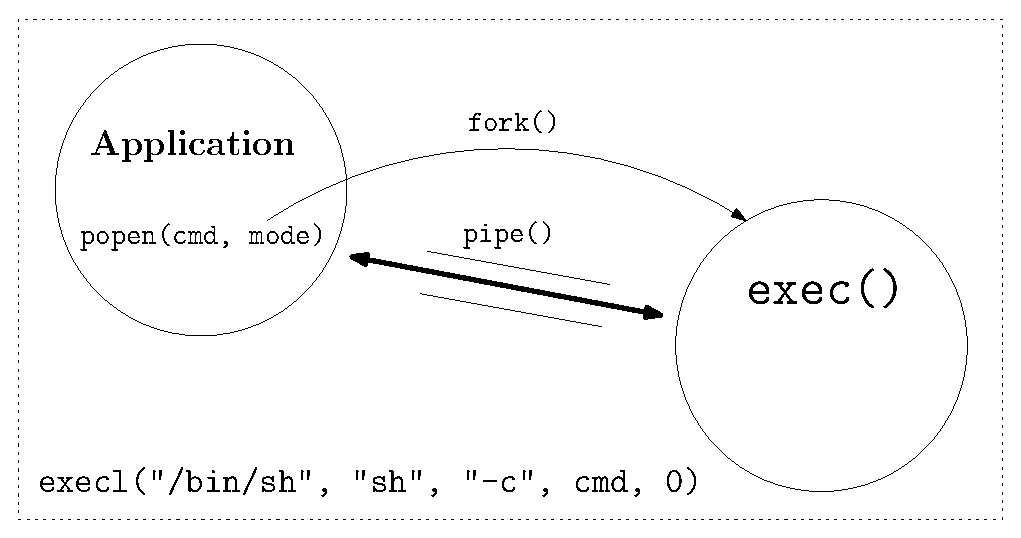
\includegraphics[width=90mm]{img/adv-ipc-and-io/popen.eps}
\end{center}


\begin{itemize}
\item As you can see from the picture, \texttt{popen()} can be used both to read
from and write data to the command. However, reading is probably the most common
case. And while it explicitly says ,,\texttt{fork}'', it does not have to be
like that, of course. The implementation is system depended because the UNIX
specification does not care about the actual implementation.
\item Creating a pipe, forking a new process, closing and redirecting some
descriptors -- all that is managed by the \texttt{popen()} call.
\item \texttt{FILE *popen(const char *command, const char *mode);}\\
\texttt{int pclose(FILE *stream);}
\end{itemize}

%===============================================================================
\subsection{\texttt{popen()} and \texttt{pclose()} example code}

\begin{lstlisting}
    /* Echo the output of "ls" command to my standard
     * output. */
    FILE *ptr;
    char *cmd = "/usr/bin/ls -d *";

    if ((ptr = popen(cmd, "r")) != NULL) {
            while (fgets(buf, BUFLEN, ptr) != NULL)
                    printf("%s", buf);
    } else
            err(1, "popen");

    pclose(ptr);
\end{lstlisting}

\begin{itemize}
\item We silently assume in the code that you know how to work with a FILE type.
This was not in the [\myun\myix-prog-I] lecture. See man page for
\texttt{fopen()} and \texttt{fclose()} if needed.
\item If you use threads, you should use \texttt{popen}/\texttt{pclose} instead
of thread unsafe \texttt{system(3c)}.
\item \priklad{adv-ipc-and-io/popen.c}
\item \emsl{Exercise:} modify the code so that you feed your standard input
through:\\ \texttt{tr [[:alpha:]] [[:upper:]]} using \texttt{popen()}. Print the
output of \texttt{tr} on the standard output of your program.
\end{itemize}

%===============================================================================
\subsection{Mechanisms for Creating a Process}

We know functions that somehow create a process for us:

\begin{itemize}
\item \texttt{fork(void)}
\item \texttt{fork\_all(void)}
	\begin{itemize}
	\item forks and duplicates all existing threads. That was the former
	default behaviour of Solaris threads, \texttt{fork\_all()} now exists
	to allow backward compatibility.
	\end{itemize}
\item \texttt{popen(const char *command, const char *mode)}
\item \texttt{system(const char *string)}
\end{itemize}

Now we add a new one:
\begin{itemize}
\item \texttt{posix\_spawn(...)}
\end{itemize}

\begin{itemize}
\item \texttt{fork\_all()} was already mentioned in [\myun\myix-prog-I].
\end{itemize}

%===============================================================================
\subsection{\texttt{posix\_spawn()}, \texttt{posix\_spawnp()}}

\begin{itemize}
\item creating a new process from a process image in a single step
	\begin{itemize}
	\item no need for a fork and exec in the program itself
	\item HW architectures w/o dynamic address translation can not easily
	provide \texttt{fork()} since the addresses in the process are physical
	addresses
	\end{itemize}
\item it is part of POSIX real time extensions (POSIX.1d), see [posix.1d]
\item note that there must be means to specify various attributes normally dealt
with after \texttt{fork()} but before \texttt{exec()}
	\begin{itemize}
	\item user/group ID changes, signal mask and file descriptor
	manipulations
	\end{itemize}
\end{itemize}

\begin{itemize}
\item See [\myun\myix-prog-I] for more info on the POSIX standards.
\end{itemize}

%===============================================================================
\subsection{Using \texttt{posix\_spawn()}}

\begin{tabbing}
int \funnm{posix\_spawn}(\=pid\_t *restrict \emph{pid},\\
		\>const char *restrict \emph{path},\\
		\>const posix\_spawn\_file\_actions\_t *\emph{file\_actions},\\
		\>const posix\_spawnattr\_t *restrict \emph{attrp},\\
		\>char *const \emph{argv}[restrict],\\
		\>char *const \emph{envp}[restrict]);
\end{tabbing}

\begin{itemize}
\item \texttt{posix\_spawnp()} function call is the same as
\texttt{posix\_spawn()} but \texttt{PATH} is used if the \texttt{path} argument
does not contain a slash
\item you need \texttt{path} and \texttt{argv}, everything else can be set to
\texttt{NULL}
\item however, to read from a pipe, for example, you will need to use \emph{file
actions}
\end{itemize}

\begin{itemize}
\item The \emph{pid} will be filled with the child's PID.
\item \emph{attrp} contains various attributes applied on the process like
user/group IDs, signal masks, process group membership, ...
\item File actions contains info on how to deal with individual file descriptors
(if needed). If \texttt{NULL}, the behaviour will be the same as with
\texttt{fork()}, including honoring the \texttt{FD\_CLOEXEC} flag.
\item \emph{argv} is mandatory, with at least \texttt{argv[0]} (+
\texttt{argv[1]} containing NULL).
\end{itemize}

%===============================================================================
\subsection{File actions}

\begin{itemize}
\item if you want to duplicate the standard output to a pipe in the child, for
example, you must use file actions
\end{itemize}

\begin{lstlisting}
posix_spawn_file_actions_t factions;

pipe(p);
flags = fcntl(p[0], F_GETFL);
/* FD_CLOEXEC works together with file actions. */
fcntl(p[0], F_SETFL, flags | FD_CLOEXEC);
posix_spawn_file_actions_init(&factions);
posix_spawn_file_actions_adddup2(&factions, p[1], 1);
posix_spawn_file_actions_addclose(&factions, p[1]));
\end{lstlisting}


\begin{itemize}
\item File actions are performed in the child in the order in which they were
added to the file action object. File actions are performed before file
descriptors tagged with the \texttt{FD\_CLOEXEC} flag are closed.
\item One more file action you can use is
\texttt{posix\_spawn\_file\_actions\_addclose}.
\item \priklad{adv-ipc-and-io/posix\_spawn.c}
\item \emsl{Exercise:} change the code so that the new process blocks
\texttt{SIGTERM} signal, then call ,,\texttt{sleep 99}'' from it, and then send
it a \texttt{SIGTERM} signal from the parent. After the parent exits check that
the child is stil alive, verifying that the mask has been set properly. You will
have to use the \texttt{attrp} argument of the \texttt{posix\_spawn()}.
\end{itemize}

%===============================================================================
\subsection{Solaris Event Ports}

\begin{itemize}
\item existing ``old'' event notification frameworks
	\begin{itemize}
	\item AIO
	\item timers
	\item \texttt{poll()} 
	\end{itemize}
\item no unified way to reap an application's completion of events in Solaris
before the event ports
\item all of these frameworks built independently
\item no unified mechanism to reap events
\item varying performance and scalability of the existing frameworks
\item \emsl{need for one common API}
\end{itemize}


\label{SOLARIS_EVENT_PORTS}

\begin{itemize}
\item Solaris event ports first appeared in Solaris 10.
\item Timers were not mentioned in [\myun\myix-prog-I] nor in this material. See
\texttt{set\-i\-timer()} and \texttt{clock\_gettime()} for more information.
\end{itemize}


%===============================================================================
\subsection{Solaris Event Ports (continuted)}

\begin{itemize}
\item the fundamental piece of the event completion framework is the \emph{port}
\item applications use ports to register and reap events on the objects of
interest

\begin{lstlisting}
/* Create a port. */
int portfd = port_create();

/* Register the events you are interested in. */
port_associate(portfd,  ... );

/* Block until an event appears on the port. */
port_get(portfd,  ... );
\end{lstlisting}
\end{itemize}


\label{SOLARIS_EVENT_PORTS}

\begin{itemize}
\item Solaris event ports first appeared in Solaris 10.
\item Source code example not provided yet. See manual pages for respective functions.
\item References:
	\begin{itemize}
	\item \url{http://developers.sun.com/solaris/articles/event\_completion.html}
	\item \url{http://blogs.oracle.com/dap/entry/event\_ports\_and\_performance}
	\item \url{http://blogs.oracle.com/barts/entry/entry\_2\_event\_ports}
	\end{itemize}
\end{itemize}

%    port_create(3C), port_get(3C), ...
%    http://blogs.oracle.com/barts/entry/entry_2_event_ports
%    http://blogs.oracle.com/dap/entry/event_ports_and_performance
%    event(3) (libevent)
%    port_associate(3c) ma informace o tom, jake jsou mozne eventy
%
%    http://blogs.oracle.com/praks/entry/file_events_notification
%
%  http://blogs.oracle.com/dap/entry/libevent_and_solaris_event_ports

%===============================================================================
\subsection{FreeBSD KQueue}

\begin{itemize}
\item Kqueue is another event notification interface
\item first appeared in FreeBSD 4.1
\item Kqueue enables the user to receive alerts regarding events on specified
targets very quickly
\item ported to NetBSD and OpenBSD
\end{itemize}


\begin{itemize}
\item See \texttt{kqueue(2)} manual page on FreeBSD for more information.
\item References:
	\begin{itemize}
	\item \url{http://people.freebsd.org/~jlemon/papers/kqueue.pdf}
	\end{itemize}
\end{itemize}

%===============================================================================
\subsection{\texttt{libevent} -- a portable aproach to event notifications}

\begin{itemize}
\item asynchronous event notification software library
\item can use \texttt{/dev/poll}, Solaris event ports, kqueue,
\texttt{select()}, \texttt{poll()}, and \texttt{epoll(4)}
\item if you need an event notification framework on several different
platforms, \texttt{libevent} might be exactly what you are looking for
	\begin{itemize}
	\item should compile on Linux, *BSD, Solaris, Max OSX, and Windows
	\end{itemize}
\item written by Niels Provos
\end{itemize}


\label{LIBEVENT}

\begin{itemize}
\item \texttt{epoll(4)} is an I/O event notification facility in the Linux
kernel.
\item We already mentioned \texttt{/dev/poll} on p. \pageref{DEV_POLL}.
\item References:
	\begin{itemize}
	\item \url{http://www.monkey.org/~provos/libevent}
	\item \url{http://blogs.oracle.com/dap/entry/libevent\_and\_solaris\_event\_ports}
	\end{itemize}
\end{itemize}

\endinput
